\documentclass{article}
\usepackage{mathtools}
\usepackage{amsmath}
\usepackage{amssymb}
\usepackage{tikz}
\usepackage{lipsum}
\usepackage{graphicx}
\usepackage[finnish]{babel}
\usepackage{fancyhdr}
\usepackage{pgf,tikz}


\pagestyle{fancy}

\newcounter{tehtava}
\setcounter{tehtava}{1}


\fancyhf{}
\fancyhead[L]{Tehtävä \thetehtava}

\fancypagestyle{plain}{
    \fancyhf{}
    \fancyhead[L]{Tehtävä \thetehtava}
}

\begin{document}
    \thispagestyle{plain}
	\title{MAT11001 - Harjoitus 6}
	\date{}
	\maketitle
	
	
	\section*{Tehtävä \thetehtava}
    Jatkoa harjoituksen 5 tehtävään 5. Tarkastellaan siis kompleksilukuja $z = (3, -4)$ ja $w =(-1, 2)$
    \begin{itemize}
        \item[\textbf{a)}] Laske kompleksilukujen $z$ ja $w$ tulo
        \[
        \begin{aligned}    
            (3-4i) \cdot (-1+2i)& \\
            &= 3*(-1) + 3*2i -4i*(-1) -4i*2i \\
            &= -3 + 10i -8i^2 \quad \mid i^2 = -1 \\
            &= 5 + 10i
        \end{aligned}
        \]
        \item[\textbf{b)}] Mikä on kompleksiluvun $w$ käänteisluku? \newline
        Käytetään kaavaa
        \[
            \frac{1}{w} = \frac{1}{a + bi} = \frac{a - bi}{(a + bi)(a - bi)} = \frac{a - bi}{a^2 + b^2}
                \quad \mid
                \begin{aligned}
                &\text{Tämä johtuu siitä, että } \\ &(a + bi)(a - bi) = a^2 + b^2
                \text{on reaaliluku.}
                \end{aligned}
        \]
        Liittoluku $\overline{w} = -1 - 2i$\newline
        $\implies (w)(\overline{w}) = (-1 + 2i)(-1 - 2i) = (-1)^2 - (2i)^2 = 1 - (-4) = 5$\newline
        Tulokseksi saadaan 5 joka on reaaliarvo, jolloin $w$ käänteisluku saadaan:\newline
        \[
        \frac{1}{w} = \frac{\overline{w}}{(w)(\overline{w})} = \frac{-1 - 2i}{5} = \frac{-1}{5} - \frac{2i}{5}
        \]
        eli kompleksiluvun $w = -1 + 2i$ käänteisluku on:
        \[
            \frac{1}{w} = -\frac{1}{5} - \frac{2i}{5}
        \]
\pagebreak
        \item[\textbf{c)}] Laske kompleksilukujen $z$ ja $w$ osamäärä.\newline
        \[
            \frac{z}{w} = \frac{(z)(\overline{w})}{(w)(\overline{w})}
        \]
        Edellisestä tehtävästä näimme että $(w)(\overline{w}) = 5$ jolloin
        \[
        \begin{aligned}
            & \frac{z}{w} = \frac{(z)(\overline{w})}{5} \\
            \implies & \frac{z}{w} = \frac{(3-4i)(-1-2i)}{5} \\
            = & \frac{(-3 -6i +4i + 8i^2)}{5}
            = & \frac{-11 -2i}{5}
        \end{aligned}
        \]
    \end{itemize}

\newpage
\stepcounter{tehtava}
\section*{Tehtävä \thetehtava}
Olkoot $z = 2\sqrt{3} - 2i$ ja $w = -1 + i$
\begin{itemize}
    \item[\textbf{a)}] Määritä kompleksilukujen $z$ ja $w$ argumentit eli vaihekulmat.
    \[
        \arg(z) = \tan^{-1}\left(\frac{b}{a}\right)
    \]
    Missä $a$ on reaaliosa ja $b$ on imaginaariosa, siis:
    \[
        \arg(z) = \tan^{-1}\left(\frac{-2}{2\sqrt{3}}\right) = \tan^{-1}\left(-\frac{1}{1\sqrt{3}}\right)
    \]
    $\tan^{-1}\left(-\frac{1}{1\sqrt{3}}\right)$ vastaa $-\frac{\pi}{6}$ radiaania mistä seuraa $\arg(z) = -\frac{\pi}{6}$\newline
    \newline
    Kompleksiluvun $w = -1 + i$ argumentti:\newline
    \[
        \arg(w) = \tan^{-1}\left(\frac{1}{-1}\right) = \tan^{-1}\left(-1\right)
    \]
    $\tan^{-1}\left(-1\right)$ vastaa $-\frac{\pi}{4}$ mutta koska $w$ sijaitsee toisessa neljännekessä (negatiivinen reaaliosa, positiivinen imaginaariosa) korjaamme kulman\linebreak lisäämällä $\pi$\newline
    $\implies \pi - \frac{\pi}{4} = \frac{3\pi}{4}$\newline
    Siis $\arg(w) = \frac{3\pi}{4}$
    

    \item[\textbf{b)}] Määritä kompleksiluvun $z$ napaesitys.\newline
    
    $|z| = \sqrt{a^2 + b^2} = \sqrt{(2\sqrt{3})^2 + (-2)^2} = \sqrt{12 + 4} = \sqrt{16} = 4$ \newline
    Kohdassa a nähtiin $\arg(z) = -\frac{\pi}{6}$.\newline
    Nyt voimme kirjoittaa kompleksiluvun $z$ napaesityksen:
    \[
        z = 4 \left( \cos \left( -\frac{\pi}{6} \right) + i \sin \left( -\frac{\pi}{6} \right) \right)
    \]
    \item[\textbf{c)}] Määritä kompleksiluvun $w$ eksponenttiesitys.\newline
    $|w| = \sqrt{a^2 + b^2} = \sqrt{(-1)^2 + (1)^2} = \sqrt{1 + 1} = \sqrt{2}$\newline
    Kohdassa a nähtiin että $\arg(w) = \frac{3\pi}{4}$\newline
    Nyt voimme kirjoittaa eksponenttiesityksen:
    \[
        w = \sqrt{2} e^{i \frac{3\pi}{4}}
    \]
\end{itemize}

\newpage
\stepcounter{tehtava}
\section*{Tehtävä \thetehtava}
Olkoot $z, w \in \mathbb{C}, w \neq 0$. Osoita, että osamäärän liittoluku on liittolukujen osamäärä eli
\[
    \overline{\left(\frac{z}{w}\right)} = \frac{\overline{z}}{\overline{w}}
\]
Lasketaan ensin vasen puoli.
\[
    \begin{aligned}
        z &= a + bi \\
        w &= c + di \\
        \implies \overline{w} &= c - di \\[10pt]
        \text{Lasketaan ensin:} \\
        \left(\frac{z}{w}\right) &\implies\left(\frac{(z)(\overline{w})}{(w)(\overline{w})}\right) = \left(\frac{(a + bi)(c -di)}{(c + di)(c - di)}\right) \\
        &= \frac{ac - adi + cbi - bdi^2}{c^2 + d^2} \quad \mid i^2 = -1 \\
        &= \frac{(ac + bd) + (bc - ad)i}{c^2 + d^2} \\
        \text{Jolloin liittoluku } \overline{\left(\frac{z}{w}\right)} \text{ on:}\\
        &\frac{(ac + bd) - (bc - ad)i}{c^2 + d^2} \\
    \end{aligned}
 \]
Sitten lasketaan oikea puoli.


\[
    \begin{aligned}
        \overline{z} &= a - bi\\
        \overline{w} &= c - di\\[10pt]
        \frac{\overline{z}}{\overline{w}} &= \frac{(a - bi)(c + di)}{(c - di)(c + di)}\\
        &= \frac{ac +adi -cbi -bdi^2}{c^2 + d^2}\\
        &= \frac{(ac + bd)  + (ad -bc)i }{c^2 + d^2}\\
        &= \frac{(ac + bd)  - (bc + ad)i }{c^2 + d^2}
    \end{aligned}
\]
Eli $\overline{\left(\frac{z}{w}\right)} = \frac{\overline{z}}{\overline{w}}$ pätee.


\newpage
\stepcounter{tehtava}
\section*{Tehtävä \thetehtava}
Laske de Moivren kaavan avulla $(1 - \sqrt{3}i)^5$\newline
Lasketaan ensin kompleksiluvun napaesitys.
\[
    r = |1 - \sqrt{3}i| = \sqrt{1^2 + (-\sqrt{3})^2} = \sqrt{1 + 3} = 2
\]

\[
    arg(1 - \sqrt{3}i) = tan^{-1}\left(\frac{-\sqrt{3}}{1} \right) = tan^{-1}\left(-\sqrt{3} \right) = - \frac{\pi}{3}
\]
Koska reaaliosa on positiivinen ja imaginaariosa on negatiivinen sijaitsee kompleksiluku neljännessä neljänneksesssä eli $arg(1 - \sqrt{3}i) = - \frac{\pi}{3}$, saamme napaesityksen
\[
    \implies 2 \left( \cos\left( -\frac{\pi}{3} \right) + i \sin\left( -\frac{\pi}{3} \right) \right)
\]
Nyt de Moivren kaavalla
\[
\begin{aligned}
    (1 - \sqrt{3}i)^5 &= \left[2 \left( \cos\left( -\frac{\pi}{3} \right) + i \sin\left( -\frac{\pi}{3} \right) \right)\right]^5 \\
    &=32 \left( \cos\left( -\frac{5\pi}{3} \right) + i \sin\left( -\frac{5\pi}{3} \right) \right) \quad \mid \begin{aligned} &\text{lisätään kulmaan }2\pi \\&\text{jolloin saadaan positiivinen kulma} \end{aligned} \\
    &=32 \left( \cos\left( \frac{\pi}{3} \right) - i \sin\left( \frac{\pi}{3} \right) \right) \quad \mid \text{huomioitiin sinin parittomuus} \\
    &\text{sijoitetaan }
    \cos\left( \frac{\pi}{3} \right) = \frac{1}{2} \text{ ja } 
    \sin\left( \frac{\pi}{3} \right) = \frac{\sqrt{3}}{2} \\
    \implies 
    &32 \left( \frac{1}{2} - i \frac{\sqrt{3}}{2} \right)\\
    &= 16 - 16i\sqrt{3}
\end{aligned}
\]



\newpage
\stepcounter{tehtava}
\section*{Tehtävä \thetehtava}
Määritä \newline
(a) kompleksiluvun 1 kahdeksannet juuret, \newline
(b) kompleksiluvun i kuutiojuuret. \newline
Esitä kummankin kohdan (a) ja (b) juuret kompleksitasossa.

\begin{itemize}
    \item[\textbf{a)}]
    \[ 
        z^8 = 1 = \cos(0) + i\sin(0) = e^{i0}
    \]
    kompleksiluvun argumentti on periodinen $2\pi$:n välein joten voimme lisätä $2\pi$k argumenttiin, missä $k$ on kokonaisluku
    \[
        1 = \cos(2\pi k) + i\sin(2\pi k) = e^{i2\pi k}, \quad k \in \mathbb{Z}
    \]
    Nyt etsitään kaikki $z$ missä toteutuu
    \[
        z^8 = e^{i2\pi k}
    \]
    Otetaan kahdeksas juuri molemmilta puolilta
    \[
        z = \left( e^{i2\pi k} \right)^{\frac{1}{8}} = e^{i\frac{2\pi k}{8}} = e^{i\frac{\pi k}{4}}
    \]
    Missä \( k = 0, 1, 2, \dots, 7 \), näin saadaan juuret yhden $2\pi$:n jakson sisältä.\newline
    Lasketaan juuret $z_k$:
    \begin{itemize}
        \item[] $k = 0$:
        \[
            z_0 = e^{i\frac{\pi \times 0}{4}} = e^{i0} = \cos(0) + i\sin(0) = 1
        \]
        \item[] $k = 1$:
        \[
            z_1 = e^{i\frac{\pi}{4}} = \cos\left( \frac{\pi}{4} \right) + i\sin\left( \frac{\pi}{4} \right) = \frac{\sqrt{2}}{2} + i\frac{\sqrt{2}}{2}
        \]
        \item[] $k = 2$:
        \[
            z_2 = e^{i\frac{\pi}{2}} = \cos\left( \frac{\pi}{2} \right) + i\sin\left( \frac{\pi}{2} \right) = 0 + i \times 1 = i
        \]
        \item[] $k = 3$:
        \[
            z_3 = e^{i\frac{3\pi}{4}} = \cos\left( \frac{3\pi}{4} \right) + i\sin\left( \frac{3\pi}{4} \right) = -\frac{\sqrt{2}}{2} + i\frac{\sqrt{2}}{2}
        \]
        \item[] $k = 4$:
        \[
            z_4 = e^{i\pi} = \cos(\pi) + i\sin(\pi) = -1 + i \times 0 = -1
        \]
        \item[] $k = 5$:
        \[
            z_5 = e^{i\frac{5\pi}{4}} = \cos\left( \frac{5\pi}{4} \right) + i\sin\left( \frac{5\pi}{4} \right) = -\frac{\sqrt{2}}{2} - i\frac{\sqrt{2}}{2}
        \]
        \item[] $k = 6$:
        \[
            z_6 = e^{i\frac{3\pi}{2}} = \cos\left( \frac{3\pi}{2} \right) + i\sin\left( \frac{3\pi}{2} \right) = 0 - i = -i
        \]
        \item[] $k = 7$:
        \[
            z_7 = e^{i\frac{7\pi}{4}} = \cos\left( \frac{7\pi}{4} \right) + i\sin\left( \frac{7\pi}{4} \right) = \frac{\sqrt{2}}{2} - i\frac{\sqrt{2}}{2}
        \]
    \end{itemize}







    \iffalse
    aletaan faktoroimaan $z^8 - 1$
    \begin{itemize}
        \item[*] $z^8 - 1 = (z^4 - 1)(z^4 + 1)$
        \begin{itemize}
            \item[*] $z^4 - 1 = (z^2 - 1)(z^2 + 1)$
            \begin{itemize}
                \item[*] $z^2 - 1 = (z - 1)(z + 1)$
            \end{itemize}
            \item[*] $z^4 + 1 = (z^2 + \sqrt{2}z + 1)(z^2 - \sqrt{2}z + 1)$
        \end{itemize}
    \end{itemize}
    nyt on faktoroimalla päästy seuraavaan:
    \[
    z^8 - 1 = (z - 1)(z + 1)(z^2 + 1)(z^2 + \sqrt{2}z + 1)(z^2 - \sqrt{2}z + 1)
    \]
    ja voimme ratkaista jokaisen tekijän erikseen
    \begin{itemize}
        \item [\textbf{1.}] $z - 1 = 0$:\newline
        \[
        z = 1
        \]
        \item [\textbf{2.}] $z + 1 = 0$:\newline
        \[
        z = -1
        \]
        \item [\textbf{3.}] $z^2 + 1 = 0$:
        \[
        z^2 = -1 \implies z = \pm i
        \]
        \item [\textbf{4.}] $z^2 + \sqrt{2}z + 1 = 0$:\newline
        ratkaistaan toisen asteen yhtälö
        \[
        \begin{aligned}
            z &= \frac{-\sqrt{2} \pm \sqrt{ (\sqrt{2})^2 - 4 \times 1 \times 1 }}{2} = \frac{-\sqrt{2} \pm \sqrt{-2}}{2}\quad \mid  \sqrt{-2} = i\sqrt{2}\\
            z &= -\frac{\sqrt{2}}{2} \pm i\frac{\sqrt{2}}{2}                
        \end{aligned}
        \]
        \item [\textbf{5.}] $z^2 - \sqrt{2}z + 1 = 0$:\newline
        ratkaistaan
        \[
            \begin{aligned}
                z &= \frac{\sqrt{2} \pm \sqrt{ (\sqrt{2})^2 - 4 \times 1 \times 1 }}{2} = \frac{\sqrt{2} \pm \sqrt{2 - 4}}{2} = \frac{\sqrt{2} \pm \sqrt{-2}}{2} \quad \mid
                \begin{aligned}
                    &\text{jälleen} \\
                    &\sqrt{-2} = i\sqrt{2}
                \end{aligned} \\
            z &= \frac{\sqrt{2}}{2} \pm i\frac{\sqrt{2}}{2}
        \end{aligned}
    \]
    \end{itemize}
\fi
    Nyt voimme listata 8 juurta:
    \begin{itemize}
        \item [] \( z_0 = 1 \)
        \item [] \( z_1 = \dfrac{\sqrt{2}}{2} + i\dfrac{\sqrt{2}}{2} \)
        \item [] \( z_2 = i \)
        \item [] \( z_3 = -\dfrac{\sqrt{2}}{2} + i\dfrac{\sqrt{2}}{2} \)
        \item [] \( z_4 = -1 \)
        \item [] \( z_5 = -\dfrac{\sqrt{2}}{2} - i\dfrac{\sqrt{2}}{2} \)
        \item [] \( z_6 = -i \)
        \item [] \( z_7 = \dfrac{\sqrt{2}}{2} - i\dfrac{\sqrt{2}}{2} \)
    \end{itemize}
    \begin{center}
        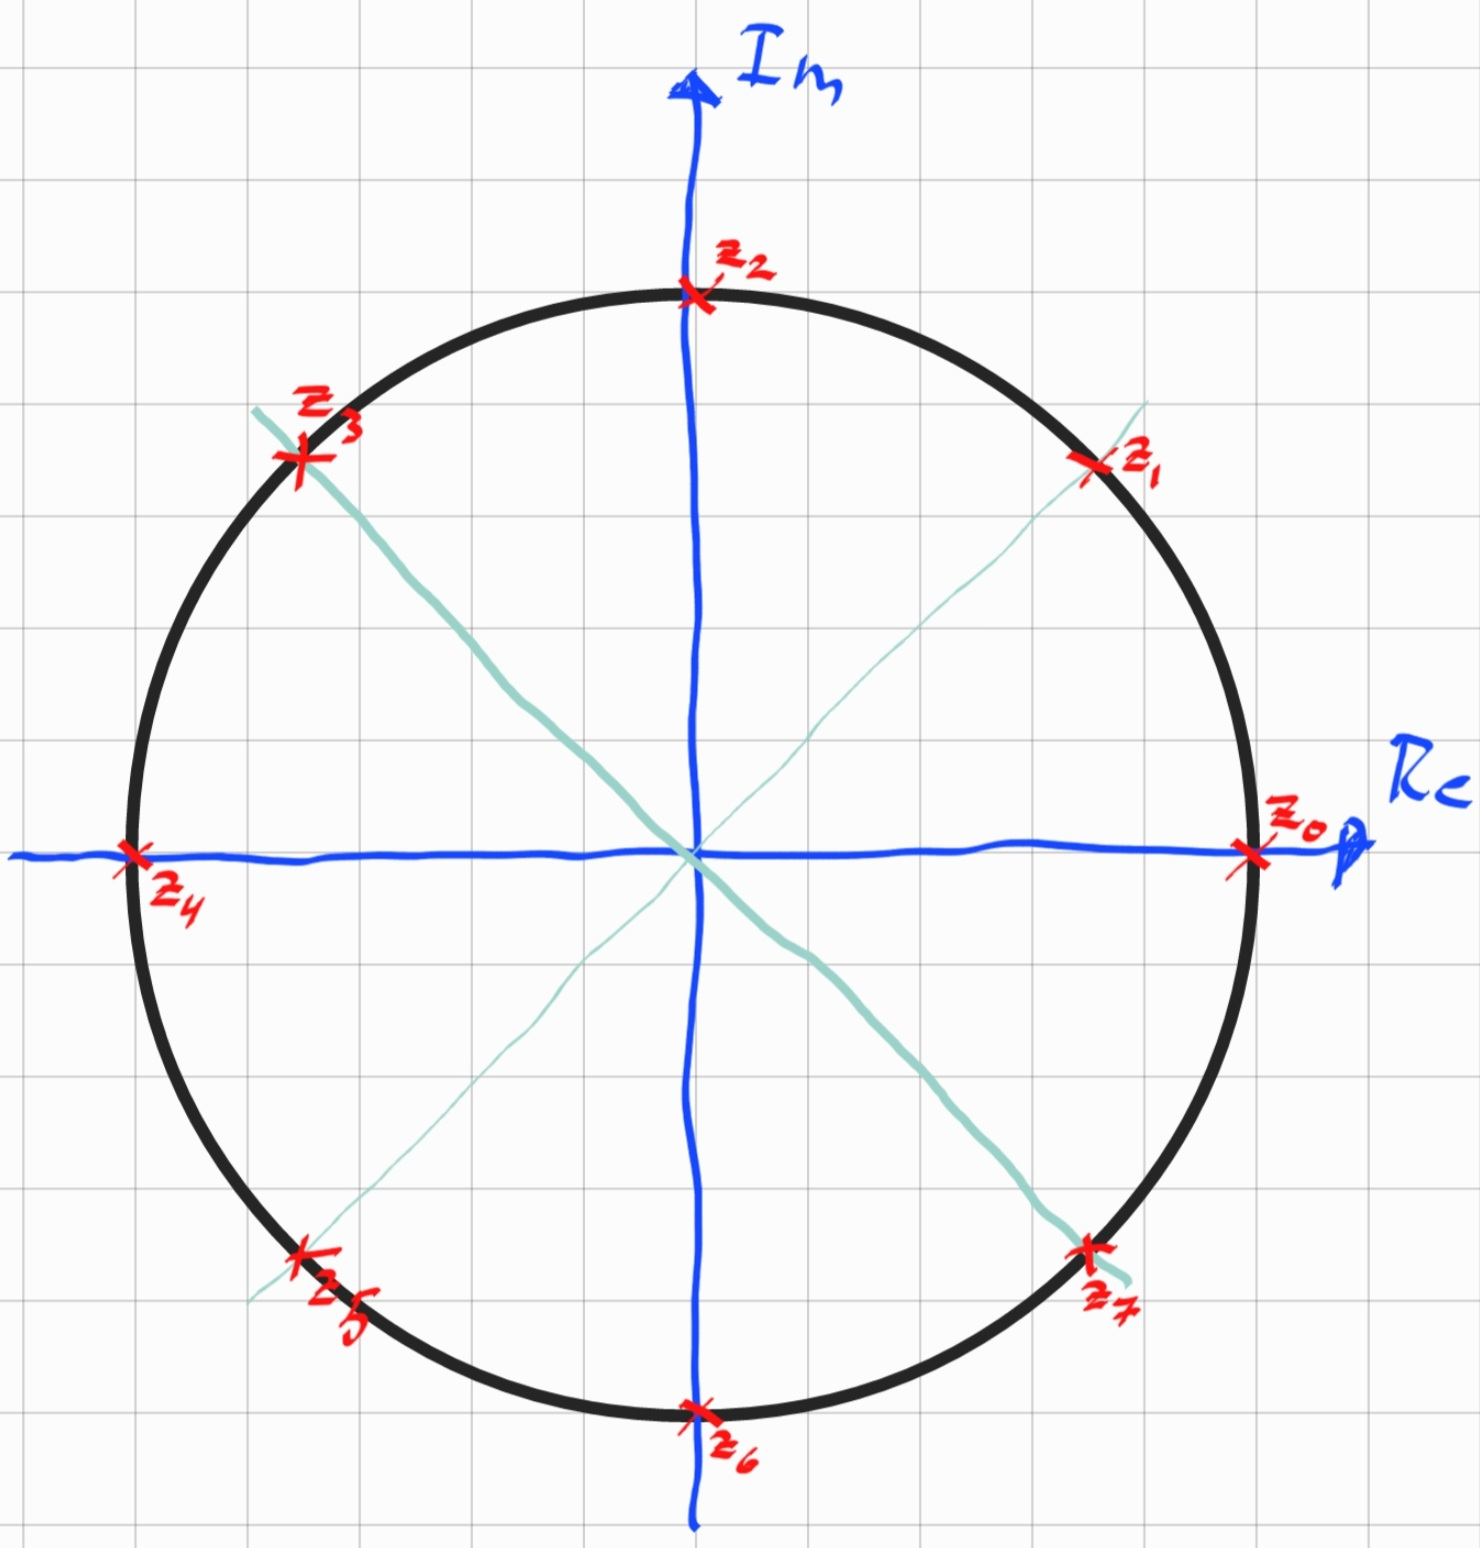
\includegraphics[width=0.7\textwidth]{harj6teht5a.jpg}
    \end{center}

    \newpage    
        
    \item[\textbf{b)}]kompleksiluvun i kuutiojuuret, siis kaikki kompleksiluvut jotka toteuttavat $z^3 = i$. \newline
    Annettu kompleksiluku $i = 0 + 1i$ joten $|z| = 1$ ja koska $i$ sijaitsee imaginaari akselilla sen argumentti on:
    \[
    \theta = \frac{\pi}{2} + 2\pi k, \quad k \in \mathbb{Z}
    \]
    lisäämällä $2\pi$k  huomioimme kulman periodisuuden.\newline
    Napamuoto:
    \[
        i = \cos\left( \frac{\pi}{2} + 2\pi k \right) + i \sin\left( \frac{\pi}{2} + 2\pi k \right)
    \]
    Seuraavaksi esitetään tuntematon kompleksiluku $z$ napamuodossa:
    \[
    z = r \left( \cos \phi + i \sin \phi \right)
    \]
    Sovelletaan de Moivren kaavaa yhtälön $z^3 = i$ kanssa
    \[
    z^3 = \left[ r \left( \cos \phi + i \sin \phi \right) \right]^3 = r^3 \left( \cos 3\phi + i \sin 3\phi \right) = \cos\left( \frac{\pi}{2} + 2\pi k \right) + i \sin\left( \frac{\pi}{2} + 2\pi k \right)
    \]
    \textbf{Itseisarvojen ja argumenttien yhtälöt}
    \[
    r^3 = 1 \implies r = 1
    \]
    Argumenttien yhtäsuuruus
    \[
    3\phi = \frac{\pi}{2} + 2\pi k, \quad k \in \mathbb{Z}
    \]
    josta ratkaistaan $\phi$
    \[
    \phi = \frac{1}{3} \left( \frac{\pi}{2} + 2\pi k \right) = \frac{\pi}{6} + \frac{2\pi k}{3}
    \]
    Argumentti on periodinen $2\pi$:n välein, siis riittää kokeilla $k = 0, 1, 2$ jotta saadaan kaikki juuret täyden kierroksen sisältä.
    \begin{itemize}
        \item[k = 0:]
        \[
        \phi_0 = \frac{\pi}{6} + \frac{2\pi \times 0}{3} = \frac{\pi}{6}
        \]
        \item[k = 1:]
        \[
        \phi_1 = \frac{\pi}{6} + \frac{2\pi \times 1}{3} = \frac{\pi}{6} + \frac{2\pi}{3} = \frac{\pi}{6} + \frac{4\pi}{6} = \frac{5\pi}{6}
        \]
        \item[k = 2:]
        \[
        \phi_2 = \frac{\pi}{6} + \frac{2\pi \times 2}{3} = \frac{\pi}{6} + \frac{4\pi}{3} = \frac{\pi}{6} + \frac{8\pi}{6} = \frac{9\pi}{6} = \frac{3\pi}{2}
        \]
    \end{itemize}
\newpage
    $r$ oli 1 jotan $z_k$ saadaan suoraan $z_k = \cos \phi_k + i \sin \phi_k$
    \begin{itemize}
        \item [1.] Juuri (k = 0)
        \[
        \begin{aligned}
            \phi_0 &= \frac{\pi}{6}\\
            \implies z_0 &= \cos\left( \frac{\pi}{6} \right) + i \sin\left( \frac{\pi}{6} \right) = \frac{\sqrt{3}}{2} + i \frac{1}{2}
        \end{aligned}
        \]
        \item [2.] Juuri (k = 1)
        \[
        \begin{aligned}
            \phi_1 &= \frac{5\pi}{6}\\
            \implies z_1 &= \cos\left( \frac{5\pi}{6} \right) + i \sin\left( \frac{5\pi}{6} \right) = -\frac{\sqrt{3}}{2} + i \frac{1}{2}
        \end{aligned}
        \]
        \item [3.] Juuri (k = 2)
        \[
        \begin{aligned}
            \phi_2 &= \frac{3\pi}{2}\\
            \implies z_2 &= \cos\left( \frac{3\pi}{2} \right) + i \sin\left( \frac{3\pi}{2} \right) = 0 - i = -i            
        \end{aligned}
        \]
    \end{itemize}
    \begin{center}
        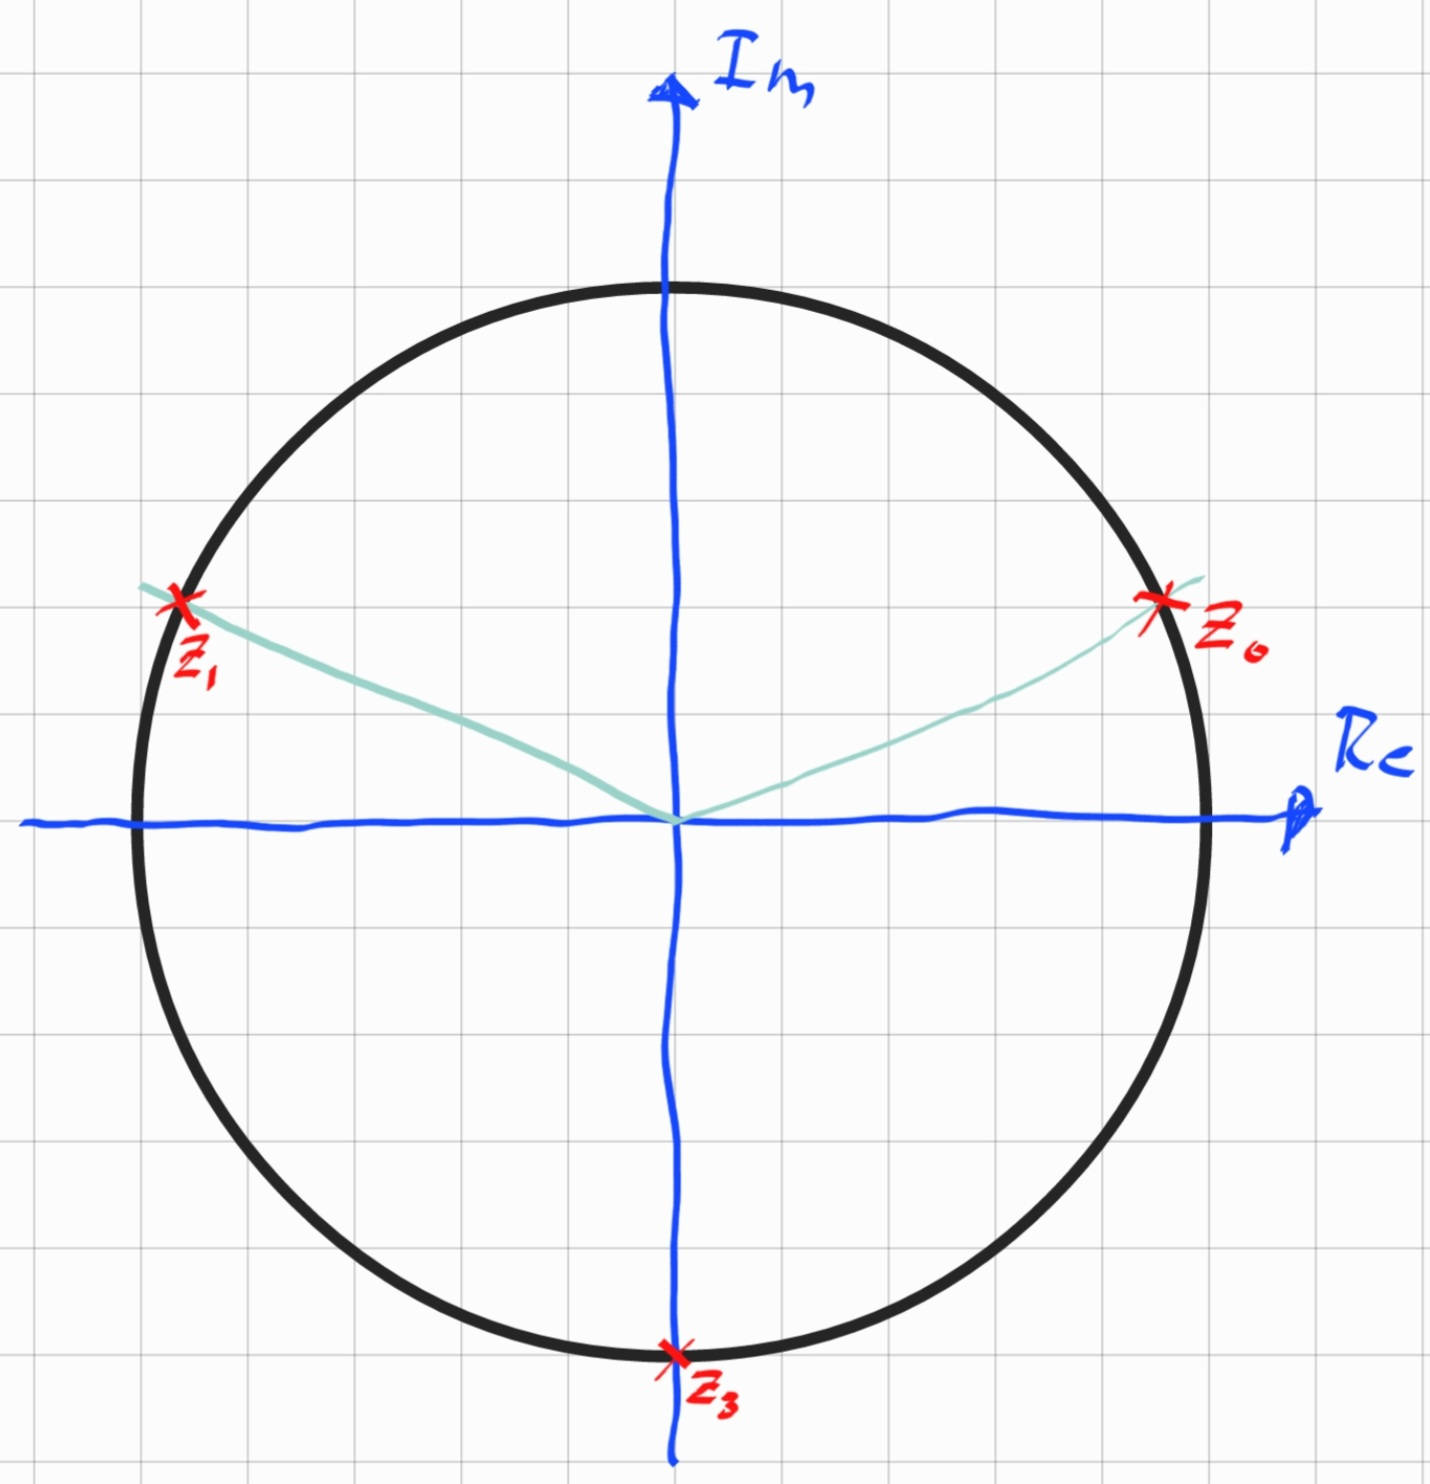
\includegraphics[width=0.7\textwidth]{harj6teht5b.jpg}
    \end{center}
\end{itemize}

\newpage
\stepcounter{tehtava}
\section*{Tehtävä \thetehtava}
Ratkaise kompleksilukujen joukossa yhtälöt\newline
(a) $x^2 + 2x + 5 = 0$\newline
(b) $x^4 - 2x^2 + 4 = 0$\newline
Esitä kummankin kohdan (a) ja (b) ratkaisut kompleksitasossa.

\begin{itemize}
    \item [{\textbf{a)}}] $x^2 + 2x + 5 = 0$ on toisen asteen yhtälö, eleisessä muodossa $ax^2 + bx + c = 0$ 
    missä $a = 1, b = 2, c = 5$\newline
    Lasketaan diskriminantti $D = b^2 - 4ac$
    \[
        D = (2)^2 - 4 \times 1 \times 5 = 4 - 20 = -16
    \]
    Koska diskriminantti on negatiivinen ei ole olemassa reaalisia ratkaisuja mutta voi olla kompleksilukujen joukossa.
    \[
        \sqrt{D} = \sqrt{-16} = 4i
    \]
    sijoitetaan arvot toisen asteen yhtälön ratkaisukaavaan
    \[
        x = \frac{-b \pm \sqrt{D}}{2a} = \frac{-2 \pm 4i}{2 \times 1} = \frac{-2 \pm 4i}{2} = -1 \pm 2i
    \]
    Tästä nähdään että yhtälön ratkaisut ovat $-1 + 2i$ ja $-1 - 2i$

    \begin{center}
        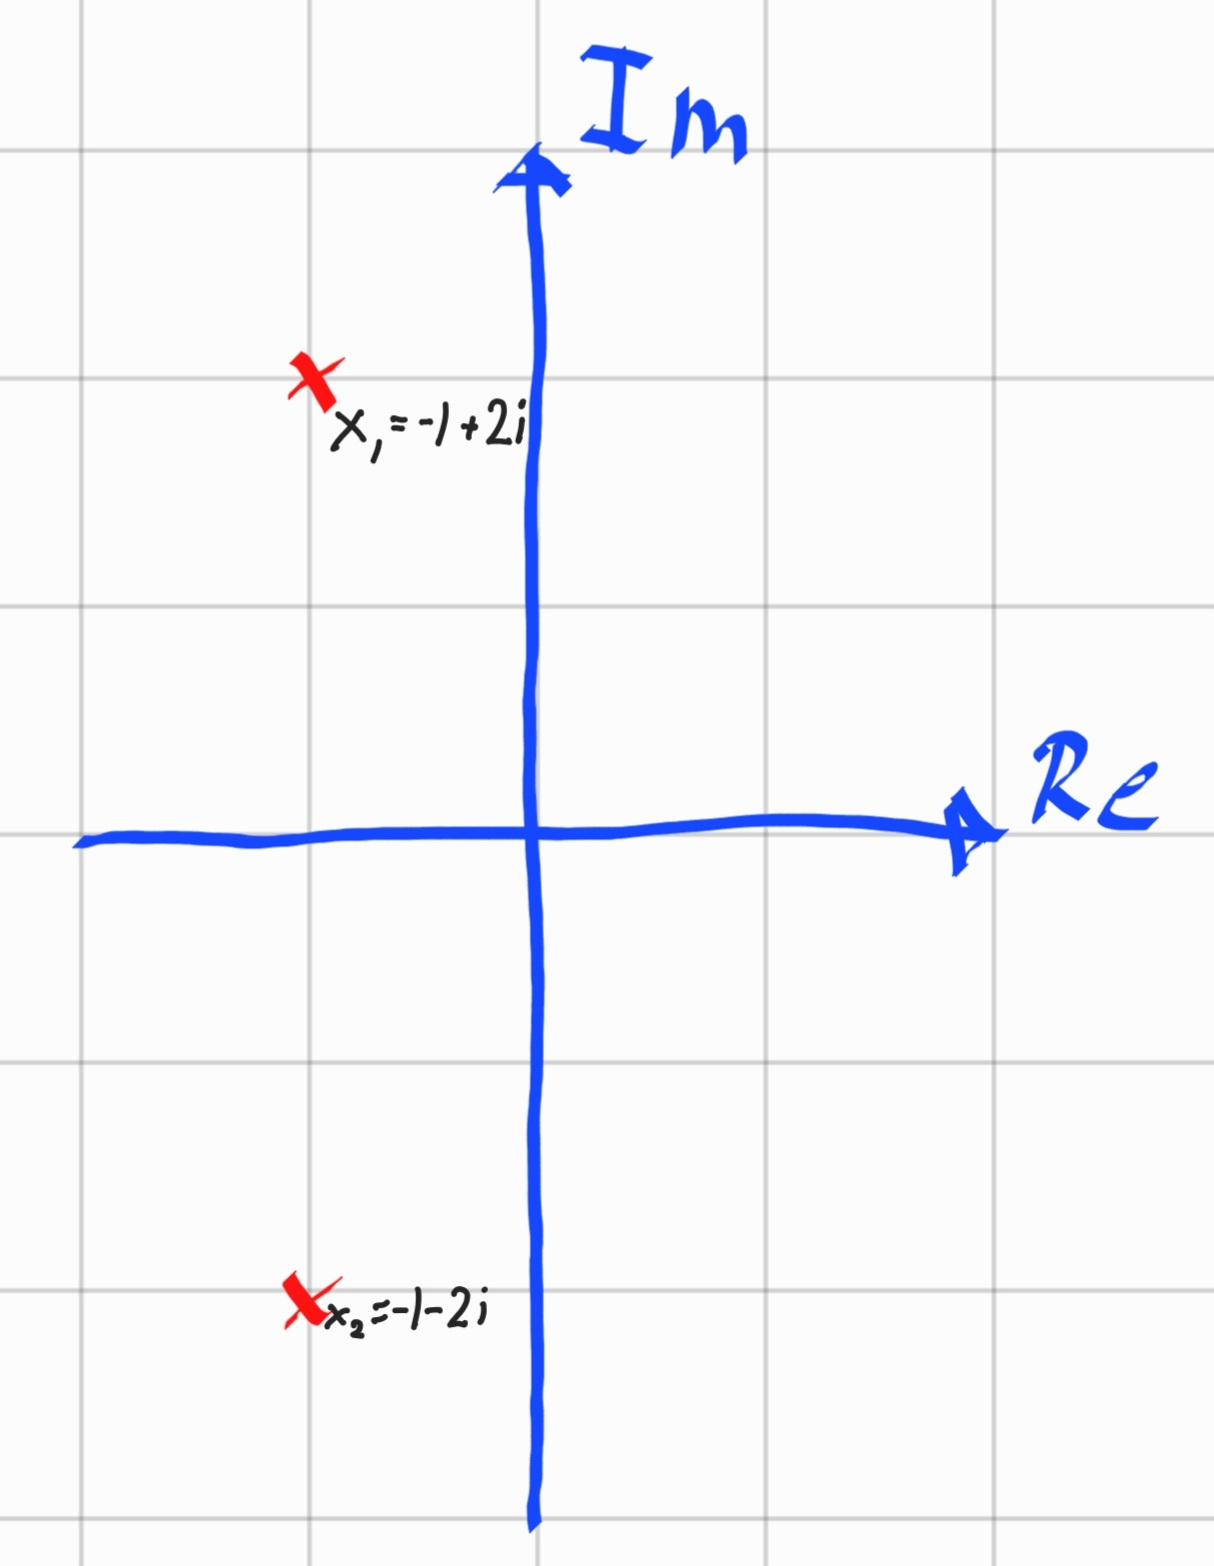
\includegraphics[width=0.5\textwidth]{harj6teht6a.jpg}
    \end{center}


\newpage
    \item [{\textbf{b)}}] $x^4 - 2x^2 + 4 = 0$ \newline
    Kirjoitetaan $y = x^2$ jolloin yhtälö muuttuu muotoon $y^2 - 2y + 4 = 0$ ja käytetään toisen asteen yhtölän ratkaisukaavaa:
    \[
    y = \frac{-b \pm \sqrt{b^2 - 4ac}}{2a}
    \]
    missä arvoilla $a=1, b=-2, c=4$ lasketaan diskriminantti:
    \[
    D = b^2 - 4ac = (-2)^2 - 4 \times 1 \times 4 = 4 - 16 = -12
    \]
    Koska $D$ on negatiivinen saadaan kompleksiset juuret
    \[
        \sqrt{D} = \sqrt{-12} = \sqrt{12} \cdot i = 2\sqrt{3} \cdot i
    \]
    ratkaistaan $y$
    \[
    y = \frac{-(-2) \pm 2\sqrt{3} i}{2 \times 1} = \frac{2 \pm 2\sqrt{3} i}{2} = 1 \pm \sqrt{3} i
    \]
    eli $y$ saa arvot
    \begin{itemize}
        \item[] $y_1 = 1 + \sqrt{3} i$
        \item[] $y_2 = 1 - \sqrt{3} i$
    \end{itemize}
    ja yritetään ratkaista $x$ jokaiselle $y$:
    \begin{itemize}
        \item[] $x^2 = y_1$
        \item[] $x^2 = y_2$
    \end{itemize}
    \textbf{Ratkaistaan $x^2 = y_1$}:\newline
    Määritetään $y_1$ napamuodossa\newline
    \begin{itemize}
        \item itseisarvo
        \[
            |y_1| = \sqrt{1^2 + (\sqrt{3})^2} = \sqrt{1 + 3} = 2
        \]
        \item argumentti
        \[
            \theta = tan^{-1}\left( \frac{\sqrt{3}}{1} \right) = \frac{\pi}{3}
        \]
    \end{itemize}
    Lasketaan $x$ käyttämällä neliöjuuren kaavaa:
    \[
        x = \sqrt{|y_1|} \left( \cos\left( \frac{\theta}{2} + k\pi \right) + i \sin\left( \frac{\theta}{2} + k\pi \right) \right), \quad k = 0, 1
    \]

    \pagebreak
    neliöjuurella on 2 arvoa:
    \begin{itemize}
        \item \textbf{k = 0:}
        \[
        \begin{aligned}            
            x &= \sqrt{2} \left( \cos\left( \frac{\pi}{6} \right) + i \sin\left( \frac{\pi}{6} \right) \right) \quad \mid
            \begin{aligned}
                \cos\left( \frac{\pi}{6} \right) &= \frac{\sqrt{3}}{2},\\ \quad \sin\left( \frac{\pi}{6} \right) &= \frac{1}{2}
            \end{aligned}\\
            \implies 
            x &= \sqrt{2} \left( \frac{\sqrt{3}}{2} + i \frac{1}{2} \right) = \frac{\sqrt{6}}{2} + i \frac{\sqrt{2}}{2}
        \end{aligned}
        \]
        \item \textbf{k = 1:}
        \[
        \begin{aligned}
            x &= \sqrt{2} \left( \cos\left( \frac{\pi}{6} + \pi \right) + i \sin\left( \frac{\pi}{6} + \pi \right) \right) \quad \mid
            \begin{aligned}
                \cos\left( \frac{7\pi}{6} \right) &= -\frac{\sqrt{3}}{2},\\ \quad \sin\left( \frac{7\pi}{6} \right) &= -\frac{1}{2}
            \end{aligned} \\
            \implies
            x &= \sqrt{2} \left( -\frac{\sqrt{3}}{2} - i \frac{1}{2} \right) = -\frac{\sqrt{6}}{2} - i \frac{\sqrt{2}}{2}
        \end{aligned}
        \]
    \end{itemize}

    \textbf{Ratkaistaan $x^2 = y_2$}:\newline
    Määritetään $y_2$ napamuodossa\newline
    \begin{itemize}
        \item itseisarvo
        \[
            |y_2| = \sqrt{1^2 + (-\sqrt{3})^2} = 2
        \]
        \item argumentti
        \[
            \theta = \arctan\left( \frac{-\sqrt{3}}{1} \right) = -\frac{\pi}{3}
        \]
    \end{itemize}
    \pagebreak
    Lasketaan $x$ käyttämällä neliöjuuren kaavaa:
    \[
        x = \sqrt{2} \left( \cos\left( \frac{\theta}{2} + k\pi \right) + i \sin\left( \frac{\theta}{2} + k\pi \right) \right), \quad k = 0, 1
    \]



    \begin{itemize}
        \item \textbf{k = 0:}
        \[
        \begin{aligned}            
            x &= \sqrt{2} \left( \cos\left( -\frac{\pi}{6} \right) + i \sin\left( -\frac{\pi}{6} \right) \right) \quad \mid
            \begin{aligned}
                \cos\left( -\frac{\pi}{6} \right) &= \frac{\sqrt{3}}{2},\\ \quad \sin\left( -\frac{\pi}{6} \right) &= -\frac{1}{2}
            \end{aligned}\\
            \implies 
                x &= \sqrt{2} \left( \frac{\sqrt{3}}{2} - i \frac{1}{2} \right) = \frac{\sqrt{6}}{2} - i \frac{\sqrt{2}}{2}
        \end{aligned}
        \]
        \item \textbf{k = 1:}
        \[
        \begin{aligned}
            x &= \sqrt{2} \left( \cos\left( -\frac{\pi}{6} + \pi \right) + i \sin\left( -\frac{\pi}{6} + \pi \right) \right) \quad \mid
            \begin{aligned}
                \cos\left( \frac{5\pi}{6} \right) &= -\frac{\sqrt{3}}{2},\\ \quad \sin\left( \frac{5\pi}{6} \right) &= \frac{1}{2}
            \end{aligned} \\
            \implies
            x &= \sqrt{2} \left( -\frac{\sqrt{3}}{2} + i \frac{1}{2} \right) = -\frac{\sqrt{6}}{2} + i \frac{\sqrt{2}}{2}
        \end{aligned}
        \]
    \end{itemize}

    Eli, yhtälön $x^4 - 2x^2 + 4 = 0$ ratkaisut kompleksilukujen joukossa ovat:
    \begin{itemize}
        \item []\( x_1 = \dfrac{\sqrt{6}}{2} + i \dfrac{\sqrt{2}}{2} \)
        \item []\( x_2 = -\dfrac{\sqrt{6}}{2} - i \dfrac{\sqrt{2}}{2} \)
        \item []\( x_3 = \dfrac{\sqrt{6}}{2} - i \dfrac{\sqrt{2}}{2} \)
        \item []\( x_4 = -\dfrac{\sqrt{6}}{2} + i \dfrac{\sqrt{2}}{2} \)
    \end{itemize}

    \begin{center}
        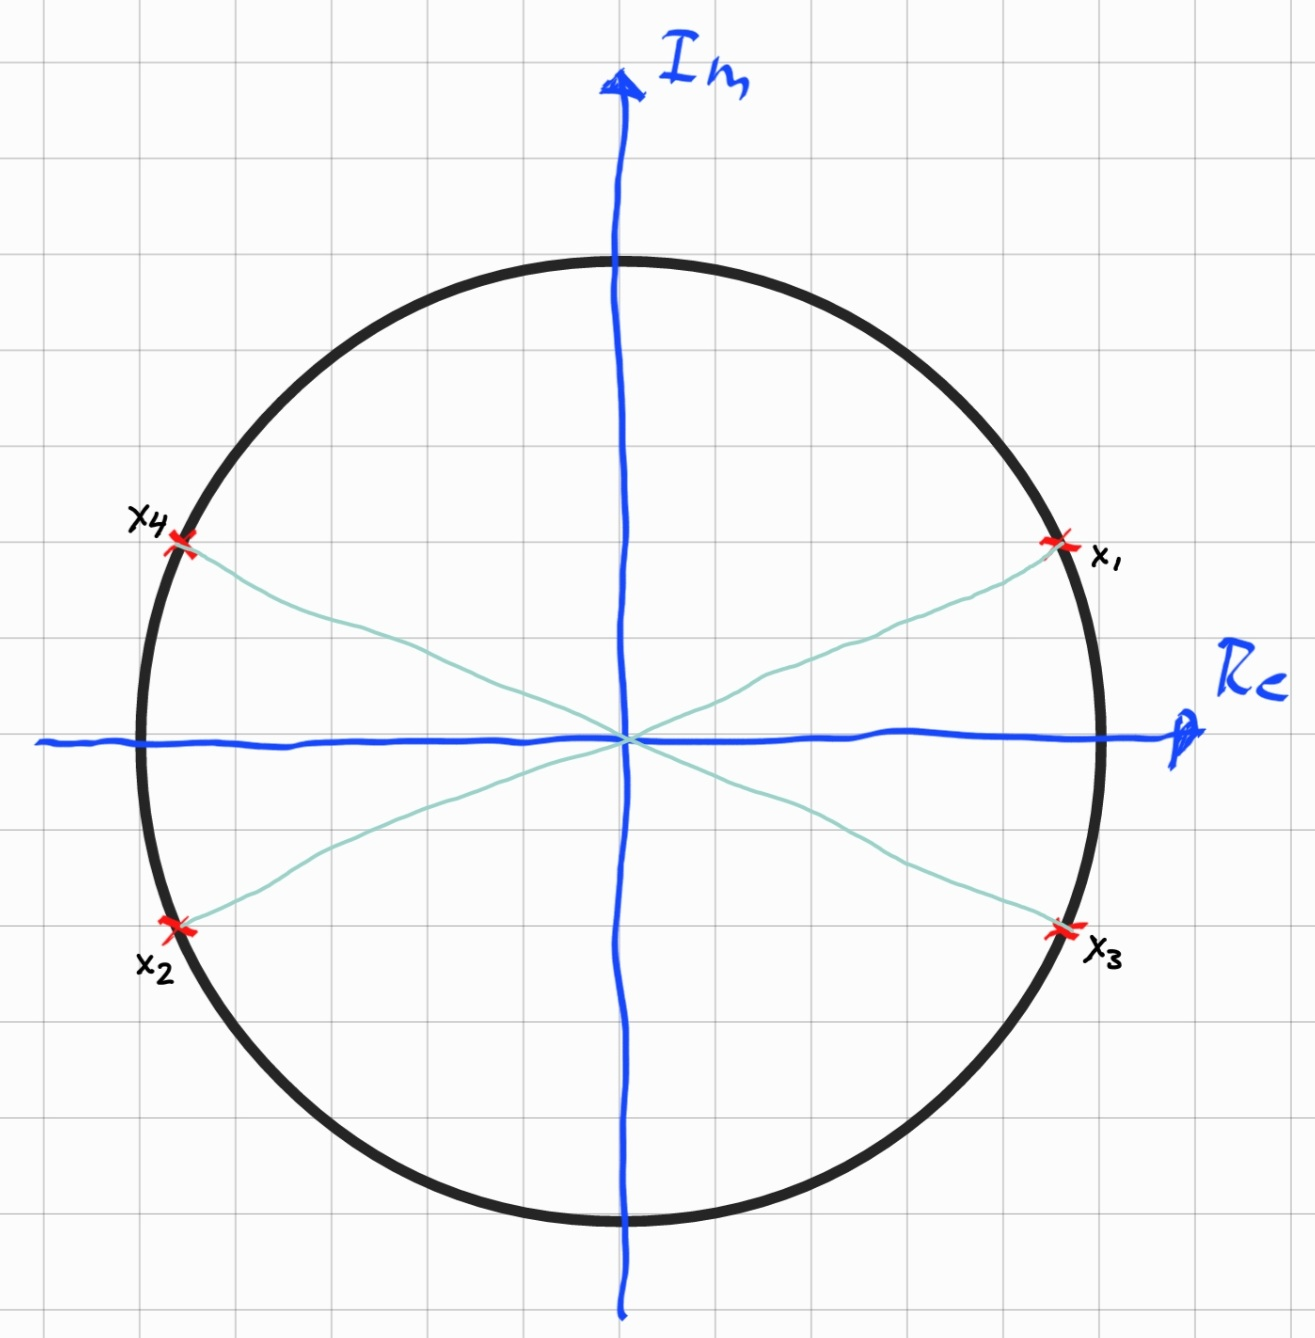
\includegraphics[width=0.45\textwidth]{harj6teht6b.jpg}
    \end{center}

\end{itemize}
\end{document}